\chapter{Formas e ângulos retos}\label{ch:g3:shapes}

Quadrados, retângulos, triângulos, círculos: as formas já são velhas
conhecidas. Este capítulo as observa com olho de geômetra --- o que
exatamente faz de um quadrado um quadrado? --- e apresenta a
ferramenta que decide: o esquadro e o seu \omterm{def:g3:shapes:rightangle}{ângulo reto}.

\section{O ângulo reto}

\begin{definition}[Ângulo reto]\label{def:g3:shapes:rightangle}
Um \emph{ângulo reto}\index{ângulo reto} é o ângulo do canto de uma
folha de papel, ou do esquadro. Duas retas que formam um ângulo reto
são \emph{perpendiculares}. Nas figuras, o ângulo reto é marcado com
um quadradinho no canto.
\end{definition}

\begin{method}[Conferir um ângulo reto]\label{met:g3:shapes:check}
\begin{enumerate}
  \item Ponha o canto do esquadro exatamente sobre o canto a testar;
  \item deslize uma das bordas do esquadro ao longo de um dos lados
        do ângulo;
  \item se o outro lado do ângulo correr exatamente ao longo da outra
        borda, o ângulo é reto --- se abrir mais ou menos, não é.
\end{enumerate}
\end{method}

\begin{omfigure}
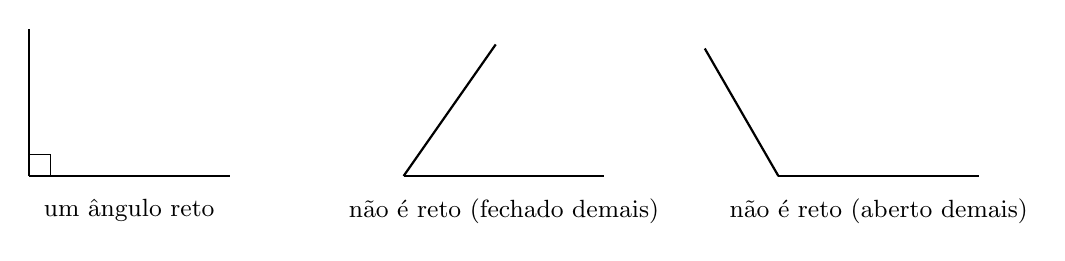
\begin{tikzpicture}[scale=0.85]
  \draw[thick] (0,0) -- (3,0);
  \draw[thick] (0,0) -- (0,2.2);
  \draw[thin] (0.32,0) -- (0.32,0.32) -- (0,0.32);
  \node[below, font=\small] at (1.5,-0.2) {um ângulo reto};
  \begin{scope}[xshift=5.6cm]
  \draw[thick] (0,0) -- (3,0);
  \draw[thick] (0,0) -- (55:2.4);
  \node[below, font=\small] at (1.5,-0.2) {não é reto (fechado demais)};
  \end{scope}
  \begin{scope}[xshift=11.2cm]
  \draw[thick] (0,0) -- (3,0);
  \draw[thick] (0,0) -- (120:2.2);
  \node[below, font=\small] at (1.5,-0.2) {não é reto (aberto demais)};
  \end{scope}
\end{tikzpicture}

{\small Só o primeiro ângulo é reto --- e só o quadradinho de marca,
ou o esquadro, pode garantir isso: os olhos sozinhos se enganam com
facilidade.}
\end{omfigure}

\section{As formas e as suas regras}

\begin{definition}[Quadrado, retângulo, triângulo]\label{def:g3:shapes:shapes}
\begin{itemize}
  \item Um \emph{retângulo}\index{retângulo} tem $4$ lados e $4$
        \omterm{def:g3:shapes:rightangle}{ângulos retos}; os seus lados opostos têm o mesmo
        comprimento.
  \item Um \emph{quadrado}\index{quadrado} é um retângulo cujos $4$
        lados têm todos o mesmo comprimento.
  \item Um \emph{triângulo}\index{triângulo} tem $3$ lados; um
        \emph{triângulo retângulo} tem um \omterm{def:g3:shapes:rightangle}{ângulo reto}.
  \item Um \emph{círculo}\index{círculo} é traçado com o compasso:
        todos os seus pontos estão à mesma distância (o
        \emph{raio}\index{raio}) do \emph{centro}.
\end{itemize}
\end{definition}

\begin{omfigure}
\begin{tikzpicture}[scale=0.72]
  % quadrado, marcas de ângulo reto voltadas para dentro
  \draw[thick] (0,0) rectangle (2,2);
  \foreach \x/\y/\dx/\dy in {0/0/1/1, 2/0/-1/1, 0/2/1/-1, 2/2/-1/-1}
    \draw[thin] (\x+0.22*\dx,\y) -- (\x+0.22*\dx,\y+0.22*\dy)
      -- (\x,\y+0.22*\dy);
  \draw (0.93,-0.07) -- (1.07,0.07);
  \draw (0.93,1.93) -- (1.07,2.07);
  \draw (-0.07,0.93) -- (0.07,1.07);
  \draw (1.93,0.93) -- (2.07,1.07);
  \node[below, font=\small] at (1,-0.35) {quadrado};
  % retângulo
  \begin{scope}[xshift=3.8cm]
  \draw[thick] (0,0) rectangle (3,2);
  \foreach \x/\y/\dx/\dy in {0/0/1/1, 3/0/-1/1, 0/2/1/-1, 3/2/-1/-1}
    \draw[thin] (\x+0.22*\dx,\y) -- (\x+0.22*\dx,\y+0.22*\dy)
      -- (\x,\y+0.22*\dy);
  \node[below, font=\small] at (1.5,-0.35) {retângulo};
  \end{scope}
  % triângulo retângulo
  \begin{scope}[xshift=8.6cm]
  \draw[thick] (0,0) -- (2.6,0) -- (0,2) -- cycle;
  \draw[thin] (0.28,0) -- (0.28,0.28) -- (0,0.28);
  \node[below, font=\small] at (1.3,-0.35) {triângulo retângulo};
  \end{scope}
  % círculo
  \begin{scope}[xshift=13.2cm]
  \draw[thick] (1,1) circle (1.1);
  \fill (1,1) circle (1.5pt);
  \draw[omDef, thick] (1,1) -- ++(45:1.1);
  \node[omDef, font=\small, above right] at (1.72,1.68) {raio};
  \node[below, font=\small] at (1,-0.35) {círculo};
  \end{scope}
\end{tikzpicture}

{\small A galeria de formas, com as suas marcas: quadradinhos para os
\omterm{def:g3:shapes:rightangle}{ângulos retos}, tracinhos para os lados iguais.}
\end{omfigure}

\begin{example}[Por que as marcas importam]\label{ex:g3:shapes:marks}
Uma forma desenhada um pouco inclinada pode \emph{parecer} um
quadrado sem ser um. As marcas dizem a verdade: $4$ quadradinhos de
\omterm{def:g3:shapes:rightangle}{ângulo reto} $+$ $4$ tracinhos $=$ um quadrado de verdade. Quando
desenhar, ponha as marcas; quando ler uma figura, confie apenas nas
marcas e nas medidas dadas.
\end{example}

\section{Desenhar no papel quadriculado}

\begin{method}[Construções na malha]\label{met:g3:shapes:grid}
O papel quadriculado oferece \omterm{def:g3:shapes:rightangle}{ângulos retos} de graça: as suas linhas
são perpendiculares.
\begin{enumerate}
  \item Para desenhar um retângulo $5$ por $3$: escolha um cruzamento,
        conte $5$ quadradinhos para a direita e $3$ para cima, e feche
        a forma pelas linhas da malha;
  \item para conferir comprimentos iguais, conte quadradinhos;
  \item passos na diagonal fazem linhas inclinadas: repetir ``$1$
        para a direita, $1$ para cima'' traça uma reta de
        $45^\circ$.
\end{enumerate}
\end{method}

\begin{omfigure}
\begin{tikzpicture}[scale=0.5]
  \draw[gray!40, thin] (0,0) grid (13,5);
  \draw[very thick, omDef] (1,1) rectangle (6,4);
  \draw[very thick, omThm] (8,1) -- (12,1) -- (8,4) -- cycle;
  \node[omDef, font=\small, below] at (3.5,-0.15)
    {retângulo $5 \times 3$};
  \node[omThm, font=\small, below] at (10,-0.15) {triângulo retângulo};
\end{tikzpicture}

{\small Duas construções na malha: as linhas da malha garantem os
\omterm{def:g3:shapes:rightangle}{ângulos retos}.}
\end{omfigure}

\begin{example}[Um programa de construção]\label{ex:g3:shapes:program}
Uma figura pode ser descrita por instruções: ``1. Trace um quadrado
$ABCD$ de lado $4$ cm. 2. Trace o círculo de centro $A$ que passa por
$B$.'' Seguindo um programa linha por linha, qualquer pessoa redesenha
a mesma figura --- e escrever um deles obriga a dar nome a cada
ponto. Experimente em dupla: um escreve, o outro desenha.
\end{example}

\section{Exercícios}

\begin{exercise}[$\star$]\label{exo:g3:shapes:1}
Na sala de aula, encontre (sem medir) três \omterm{def:g3:shapes:rightangle}{ângulos retos} e um ângulo
que não seja reto. Como você pode \emph{conferir} cada um deles?
\end{exercise}

\begin{exercise}[$\star$]\label{exo:g3:shapes:2}
Trace um retângulo de $6$ cm por $4$ cm com régua e esquadro. Marque
os seus \omterm{def:g3:shapes:rightangle}{ângulos retos} e os seus lados iguais.
\end{exercise}

\begin{exercise}[$\star$]\label{exo:g3:shapes:3}
Trace um quadrado de lado $5$ cm. Quantos \omterm{def:g3:shapes:rightangle}{ângulos retos} ele tem?
Quantos lados iguais? Marque tudo.
\end{exercise}

\begin{exercise}[$\star$]\label{exo:g3:shapes:4}
No papel quadriculado, desenhe: um quadrado $4 \times 4$; um
retângulo $7 \times 2$; um triângulo retângulo com catetos de $3$ e
$5$ quadradinhos.
\end{exercise}

\begin{exercise}[$\star$]\label{exo:g3:shapes:5}
Verdadeiro ou falso? Explique.
``Todo quadrado é um retângulo.'' \quad
``Todo retângulo é um quadrado.'' \quad
``Um triângulo pode ter dois \omterm{def:g3:shapes:rightangle}{ângulos retos}.'' (Tente desenhar um!)
\end{exercise}

\begin{exercise}[$\star$]\label{exo:g3:shapes:6}
Trace um círculo de \omterm{def:g3:shapes:shapes}{raio} $4$ cm. Marque o seu centro $O$, um ponto
$A$ sobre o círculo, e trace o \omterm{def:g3:shapes:shapes}{raio} $[OA]$. Quanto mede $OA$? E se
$B$ for outro ponto do círculo, quanto mede $OB$?
\end{exercise}

\begin{exercise}[$\star$]\label{exo:g3:shapes:7}
Siga este programa: ``1. Trace um retângulo $ABCD$ com $AB = 6$ cm e
$BC = 3$ cm. 2. Marque o ponto $M$ no meio de $[AB]$. 3. Ligue $M$ a
$C$ e a $D$.'' Em que formas o retângulo ficou dividido?
\end{exercise}

\begin{exercise}[$\star$]\label{exo:g3:shapes:8}
Separe as formas: quais destas têm pelo menos um \omterm{def:g3:shapes:rightangle}{ângulo reto}? Um
quadrado; um retângulo (não quadrado); um triângulo retângulo; um
círculo; a letra L desenhada com traços grossos.
\end{exercise}

\begin{exercise}[$\star\star$]\label{exo:g3:shapes:9}
No papel quadriculado, desenhe um quadrado inclinado cujos lados
sigam ``$2$ para a direita, $1$ para cima'' (e as viradas
correspondentes). Conte quadradinhos para se convencer de que os
quatro lados têm o mesmo comprimento.
\end{exercise}

\begin{exercise}[$\star\star$]\label{exo:g3:shapes:10}
Escreva um programa de construção (instruções numeradas, pontos com
nome) para: um quadrado de lado $3$ cm apoiado em cima de um
retângulo de $3$ cm $\times$ $2$ cm, como uma casa sobre o seu térreo.
Teste o seu programa com um colega.
\end{exercise}

\begin{exercise}[$\star\star$]\label{exo:g3:shapes:11}
Quantos quadrados você consegue encontrar numa malha $3 \times 3$ de
quadradinhos? (Conte os $1 \times 1$, os $2 \times 2$ e os
$3 \times 3$.)
\end{exercise}
